\documentclass[a4paper, 12pt]{article}
\usepackage{amssymb}
\usepackage{amsmath}
\usepackage{graphicx}
\usepackage[section]{placeins}
\begin{document}
\author{Liam Gardner}
\title{Squaring numbers by gravity}
\date{\today}
\maketitle

\newcommand{\floor}[1]{\lfloor#1\rfloor}
\newcommand{\Mod}[2]{({#1}\operatorname{ mod } {#2})}

\section{Introduction}

When calculating powers of five, the last digit will always end in five. This can be shown in column multiplication. The rightmost column will, for a minimum power of 2, be ligned with 5s. When calculating, we know that $5\cdot5 = 25$. The two is carried over to the next column over whilst the five remains. When looking at powers of five, specifically 5 to the second power. One might start to wonder what is keeping the 2 in the exponent. Since all powers of five will have the last digit of five, and since any integer greater than one, multiplied by itself must be greater than its original value, we know that at least one more digit has to come before the five. For the calculation $5^2=25$, one might remember it as the two falling and bouncing over the equal sign due to gravity, as seen in figure 1. Though for some it may be a nice way of remembering a simple calculation, how many numbers can this be generalized to? How many numbers can be squared by ``acceleration due to gravity''?
\newline

\begin{figure}[h]
	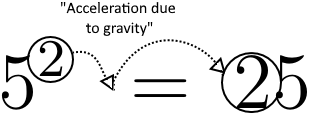
\includegraphics[scale=0.7]{Figures/Figure1.png}
	\centering
	\caption{``acceleration due to gravity.''}
	\label{fig:gravity}
\end{figure}
\FloatBarrier

\section{Defining the problem}
For any number $n^2$, if following the pattern defined above, the $2$ will be appended in front of $n$. To represent this mathematically, that is to say that $n^2 = 2\cdot10^\alpha + n$ where $\alpha$ is one more than the amount of digits in $n$. The number of digits in $n$ can be found using the base 10 logarithm. For any value $a$ such that $0\leq a \leq 9$ the base 10 logarithm will be between 0 and 1. That is to say that  $0\leq \log(a) < 1$. Since the value of the logarithm is going to be between 0 and 1, taking the closest integer less than or equal to the logarithm and addding 1 to it will return the length of the number. That is to say, for any number $n$, the amount of digits in $n$ can be calculated as $\floor{\log(n)}+1$. From this, the problem now becomes what integer values of $n$ satisfy equation 1? 
\begin{equation}
n^2=2\cdot10^{\floor{\log(n)}+1}+n
\end{equation}
\section{Solving this problem as a quadratic}
Given equation 1, if $2\cdot10^{\floor{\log(n)}+1}$ is treated as a constant then the problem becomes a quadratic and is much easier to work with. For $2\cdot10^{\floor{\log(n)}+1}$ to be considered a constant, the number of digits in $n$ must be known. If $\floor{\log(n)}+1 = 1$, or in other words, $n$ is a number such that $0\leq n \leq 9$, The solution to $n$ can be calculated as $n=\frac{1\pm\sqrt{4(20)+1}}{2}$ Since the negative solution is unimportant, the solution to this quadratic is $n=5$. What's more important is the discriminant. For $\floor{\log(n)}+1 =2$, the discriminant becomes $4(200)+1$ or $801$. If $2\cdot10^{\floor{\log(n)}+1}$ is treated as a constant, then the discriminant of the quadratic becomes $1 -4(-2\cdot10^{\floor{\log(n)}+1})$ or, expressed in a more readable format, $8\cdot10^{\floor{\log(n)}+1}+1$. For equation 1 to have any rational solutions, the discriminant must be a perfect square. To solve this, the question ``for what integer values of $n$ is $8\cdot10^{\floor{\log(n)}+1}+1$ a perfect square?'' must be answered.
\section{The perfect squares problem}
For what integer values of $n$ is $8\cdot10^{\floor{\log(n)}+1}+1$ a perfect square?
\newline
Let $r = \floor{\log(n)}+1$ so that the equation becomes $8\cdot10^r+1$. Assume that $8\cdot10^r+1$ is a perfect square and set it equal to an integer $m^2$. The equation can be rearranged to get $8\cdot10^r = (m-1)(m+1)$ From there, the base 10 logarithm can be used again to isolate for $r$, and $r$ can thus be written as a funtion of $m$ seen in equation 2.
\begin{equation}
f(m) = \log\Bigg(\frac{1}{8}(m-1)(m+1)\Bigg)
\end{equation}
Now, to answer the perfect squares question, the question ``what values of $m$ is $f(m)$ a positive integer?'' must be answered. For $f(m)$ to return a positive integer, $\frac{1}{8}(m-1)(m+1)$ must be of the form $10^k$ where $\{k\in\mathbb{Z}^+\}$. This question provides two cases. The first case is that $8|(m-1)$. The second is that $8|(m+1)$.
\subsection{Case 1, $8|(m-1)$}
Let $q = \frac{m-1}{8}$. $q(m+1)$ must now be in the form $10^k$ and thus both $(m+1)$ and $q$ must also be in that form. For $(m+1)$ to be in the form $10^k$, that would mean that all digits of $m$ are 9. $n-1$ will also be composed of all 9s aside from its last digit, which will be 8. For all positive integer values of $\beta$ where $\beta > 2$, $\Mod{10^\beta-2}{8} = 6$. For $\beta=2$, $\Mod{10^\beta-2}{8}=\Mod{98}{8}=2$. The only value of $\beta$ such that $\Mod{10^\beta-2}{8}=0$ is when $\beta=1$. For $\beta=1$, $m=10^\beta-1$ or $m=9$, which satisfies $m$ having only digits of 9. If $m=9$ then equation 2 returns the value $1$.
\subsection{Case 2, $8|(m+1)$}
If $8|m+1$ then $m-1$ must be of the form $10^k$ for some positive integer $k$. This means that $m$ is of the form $10^k+1$, and thus $m+1$ is of the form $10^k+2$. For some integer $\beta > 2$, $\Mod{10^\beta+2}{8} = 2$ For $\beta=2$, $\Mod{10^\beta+2}{8}=\Mod{102}{8}=6$ and for $\beta=1$, $\Mod{12}{8}=4$. Since no integer values of $\beta$ will make $\Mod{10^\beta+2}{8}=0$. Therefore, $8$ cannot divide into $m+1$ and thus there are no solutions.
\subsection{The perfect squares solution}
Looking at the perfect squares problem independently, $n=0$ is a solution. However, since a number cannot have 0 digits, that solution cannot apply. If $n$ could equal $0$, equation 2 would yield a perfect square of 9. When $n=1$ the perfect square generated from equation 2 is 81. Those are the only two perfect square values that exist in the range of equation 2.
\section{Conclusion}
Since the only solution for the first case of the perfect squares problem is when $r=1$ and there are no solutions to the second case. The equation $\floor{\log(n)}+1=1$ is the only answer. The only time $\floor{\log(n)}=0$ is when $0\leq\log(n)<1$ or when $n$ only has one digit. If $n$ has one digit, the determinant of the resulting quadratic from equation 1 is $1+8\cdot10$ or 81. The solution to when $0\leq n \leq 9$ is thus $\frac{1+\sqrt{81}}{2}$ or $5$. Therefore, $5$ is the only integer which can be squared by ``acceleration due to gravity''.
\end{document}